

Canards in two dimensional fast-slow systems are degenerate phenomena, while they generically occur in higher dimensional systems.
This means that while in two dimensional systems canards only occur in $O(\sqrt{\epsilon})$ in parameter space, they occur for $O(1)$ in parameter space in a three dimensional system and are therefore more robust.
In the following two sections we consider three dimensional fast slow systems with one fast and two slow variables,
\begin{equation}
\begin{cases}
\epsilon \dot{x} &=f(x,y,z,y,\epsilon),\\
\dot{y}&=g_1(x,y,z,y,\epsilon),\\
\dot{z}&=g_2(x,y,z,y,\epsilon),
\end{cases}\label{eq: fs singularity system}
\end{equation}
which fits the original form of the fast-slow system (\ref{SlowS}), with $n=1,m=2$ \citep{MMO}.
The analysis is of a similar structure as for the two dimensional case.\\

We can identify the points that will cause complication for the analysis of the system by considering the nondegeneracy conditions as in the two dimensional case. Here, the slightly extended version is
\begin{equation}
\begin{aligned}
&f(p_*,\lambda,0)=0,\\
&\pd{}{x}f(p_*,\lambda,0)=0,\\
&\pd{^2}{x^2}f(p_*,\lambda,0)\neq 0,\\
&D_{(y,z)}f(p_*,\lambda,0) \ \text{has full rank one},
\end{aligned}
\label{eq: non-degeneracy 3d system}
\end{equation}
where $ p_*=(x_*,y_*,z_*)\in F $  denotes the fold points and $ D_{(y,z)}=\left(\pd{f}{y},\pd{f}{z}\right) $  \citep{MMO}.
This gives rise to a fold line, on which all of the fold points, $p_*$, lie.
This consequence is immediately obvious by considering Figure \ref{fig: 3d folded singularity}, and taking the two dimensional Van der Pol system as a crosssection of the two dimensional plane. Then the two fold points in the two dimensional case extend to two fold lines in the three dimensional case.
\begin{figure}[h!]\centering
	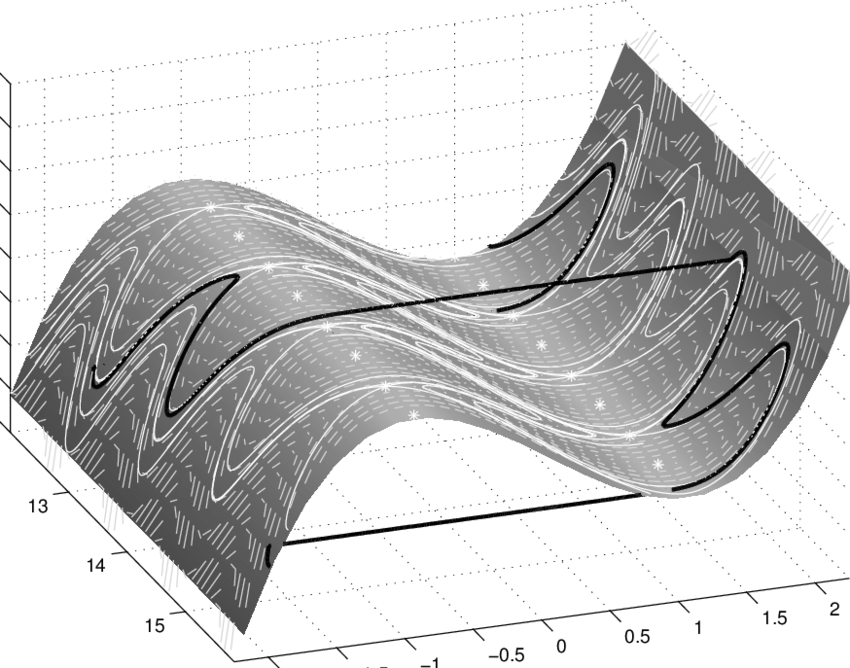
\includegraphics[height=10cm,width=14cm]{Images/Three-dimensional-plot-of-a-trajectory-for-the-van-der-Pol-equation-and-the-critical}
	\caption{Three dimensional \vdp \citep{3D-VdP}.}
	\label{fig: 3d folded singularity}
\end{figure}\newpage
In order to find the points that are classified as folded singularities, denoted by $*$ in Figure \ref{fig: 3d folded singularity}, which give rise to canard solutions, further analysis has to be carried out.
The criterion we need is the fact that a folded singularity coincides with an equilibrium of the desingularised reduced problem. Therefore, we focus on the reduced system, as in the two dimensional case. The slow system (\ref{eq: fs singularity system}) in the singular limit $\epsilon \to 0$ becomes,
\begin{equation}
\begin{cases}
0 &=f(x,y,z,y,\epsilon),\\
\dot{y}&=g_1(x,y,z,y,\epsilon),\\
\dot{z}&=g_2(x,y,z,y,\epsilon).
\end{cases}\label{eq: fs singularity systemeps0}
\end{equation}

Now, taking the total derivative of $f$ results in
\begin{align*}
0 = \od{f}{t} =\dot{y}\pd{f}{y}+\dot{z}\pd{f}{z} + \dot{x}\pd{f}{x}.
\end{align*}
Then, rearranging for the term including $\dot{x}$ and noting that $ y'=g_1 $ and $ z'=g_2 $ results in
\begin{align*}
-\dot{x}\pd{f}{x} = g_1 \pd{f}{y}+ g_2\pd{f}{z}.
\end{align*}

This is almost of the desired form, however, we cannot divide by $-\pd{f}{x}$ to get an expression for $\dot{x}$, since $\pd{f}{x}(p^*)=0$, from the nondegeneracy condition.
Therefore, as in the two dimensional case, we apply a rescaling of time in terms of $-\pd{f}{x}$, such that:
\begin{equation} \label{somegenericthreedim}
\begin{cases}
\dot{x}&=g_1\pd{f}{y}+g_2\pd{f}{z},\\
\dot{y}&=-g_1\pd{f}{x},\\
\dot{z}&=-g_2\pd{f}{x}.
\end{cases}
\end{equation}

This is the desingularised reduced system, and its equilibrium satisfies
\begin{align*}
l(p^*)= g_1(p_*,\lambda,0)\pd{}{y}f(p_*,\lambda,0)+g_2(p_*,\lambda,0)\pd{}{z}f(p_*,\lambda,0)=0.
\end{align*}
This is where the so called normal switching condition $l(p^*) \neq 0$ fails \citep{Kuehn}.
The next step is to consider the nature of the folded singularity. This was not as relevant in the two dimensional system, however, in the three dimensional case, the type of equilibrium the reduced system possesses determines the type and number of canards that can be observed in the full system.
Therefore, we consider the three dimensional Jacobian,
\begin{equation}
J=\begin{bmatrix}
\pd{\dot{x}}{x}&\pd{\dot{x}}{y}&\pd{\dot{x}}{z}\\
\pd{\dot{y}}{x}&\pd{\dot{y}}{y}&\pd{\dot{y}}{z}\\
\pd{\dot{z}}{x}&\pd{\dot{z}}{y}&\pd{\dot{z}}{z}\\
\end{bmatrix}.
\end{equation}

The resulting three eigenvalues, $ \sigma_i $ for $ i=1,2,3 $ \citep{MMO} determine the stability of the folded singularity. \Wlg we can choose $ \sigma_3=0 $ because at least one of the eigenvalues must be zero to account for the folded singularity.
The other two eigenvalues can be defined as the weak and strong eigenvalues, corresponding to the weak and strong canards, introduced below. The classification of the eigenvalues is done as follows: $ |\sigma_1|>|\sigma_2| \iff |\sigma_s|>|\sigma_w| $, i.e. the greater eigenvalue, in modulus, is defined as the strong eigenvalue and vice versa.
We can define the eigenvalue ratio $\mu:= \frac{\sigma_w}{\sigma_s}$, which will be an important +++ +++
We can infer from standard stability theory that the folded singularity can have three types of stability, classified as follows \citep{MMO},
\begin{equation}
\begin{cases}
Saddle \ \sigma_1\sigma_2<0: \sigma_i\in\R,\\
Node \ \sigma_1\sigma_2>0: \sigma_i\in\R,\\
Focus \ \sigma_1\sigma_2>0: \Im(\sigma_i)\neq 0.
\end{cases}
\end{equation}

\begin{figure}[h!]\centering
	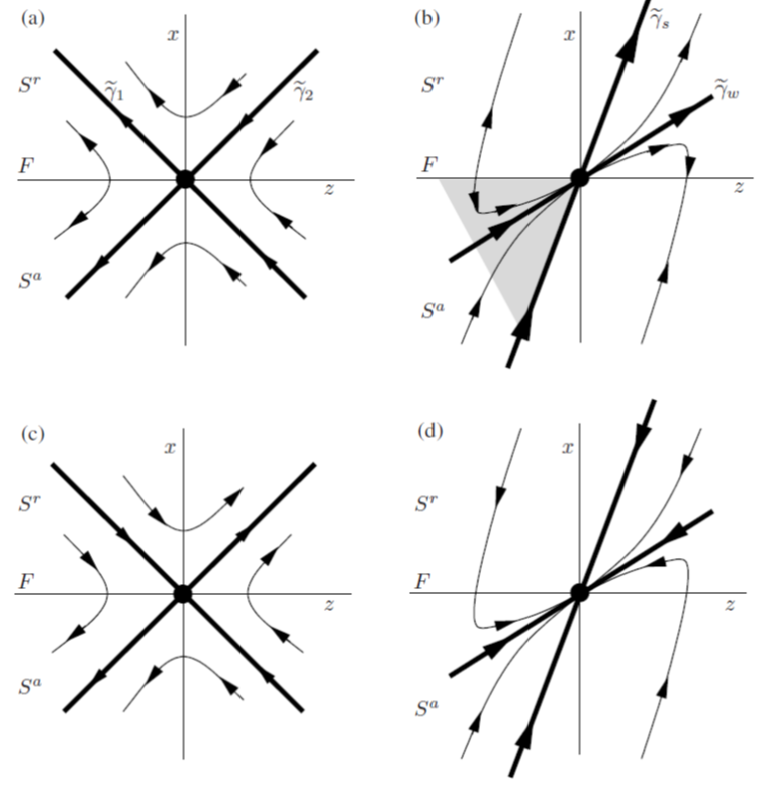
\includegraphics[height=12cm,width=12cm]{Images/foldednodesetc}
	\caption{Phase portraits around the singularities of our three dimensional system where they are a) a folded saddle and b) folded node. Corresponding desingularised flowas are shown in c) and d) \citep{MMO}.}
	\label{fig: folded singularities}
\end{figure}\newpage%arrows switch as we have reversed time
Two of the three types of equilibria are illustrated in Figure \ref{fig: folded singularities}, where the effect of the desingularisation is displayed as well. The scaling by $-\pd{f}{x}$
causes a reversal of the arrows in the repelling sheet $S^r$, which allows the two trajectories passing through the folded singularity to connect the attracting and repelling sheet which is not possible before desingularisation. These connecting trajectories are called singular canards.


\begin{figure}[h!]\centering
	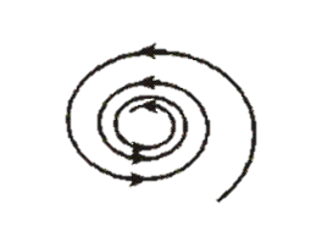
\includegraphics{Images/spiral3}
	\caption{The branches of a spiral \citep{Spiral}.}
	\label{fig: spiral}
\end{figure}\newpage

It should be noted that a singular canard is only present if the node or saddle connects the attracting and repelling sheets $ S^r $ and $ S^a $.
However, for the focus equilibrium we are unable to construct branches which connect, since the trajectories are spiralling towards or away from the equilibrium, consider Figure \ref{fig: spiral}. Then, desingularising the flow, which causes the reversal of the flow on the repelling sheet will only have the effect that the spiralling trajectories cannot cross the fold. Therefore, there are no singular canards present in the case of a folded focus.\\

The following theorem summarises the findings for the different types of equilibria and the presence of canards in three dimensions.
\begin{theorem}[Canards in $ \mathbf{R}^3$ \citep{MMO}]\label{thm: canards in R3}
	For fast-slow systems (Equation \ref{eq: fs singularity system}) with $ \epsilon>0 $ sufficiently small the following holds:
\begin{enumerate}
\item  There are no maximal canards generated by a folded focus. For a folded saddle the two singular canards $ \bar{\gamma}_{1,2} $ perturb to maximal canards $ \gamma_{1,2} $.
\item  For a folded node let $\mu=\frac{\sigma_w}{\sigma_s} <1$. the singular canard $ \bar{\gamma}_{s} $ (``the strong canard'') always perturbs to a maximal canard $ \gamma_{s} $. If $ \mu^{-1}\not \in \mathbb{N} $, then the singular canard $ \bar{\gamma}_{w} $ (``weak canard'') also perturbs to a maximal canard. We call $ \gamma_{s} $ and $ \gamma_{w} $ primary canards.
\item For a folded node suppose $ k>0 $ is an integer such that $ 2k+1<\mu^{-1} <2k+3$ and $ \mu^{-1}\neq 2(k+1) $. Then, in addition to $ \gamma_{s,w} $ there are k other maximal canards, which we call secondary canards.
\item The primary weak canard of a node undergoes a trancritical bifurcation for odd $ \mu^{-1}\in\mathbb{N} $ and a pitchfork bifurcation for even $ \mu^{-1}\in\mathbb{N} $
\end{enumerate}
\end{theorem}
This theorem summarises the findings for different types of folded singularities. It establishes the persistence of the singular canards as maximal canards of the full system $\epsilon >0$ for the different types of singularities. Furthermore, it provides a tool for caluclating the number of secondary canards present in the full system, additional to the primary canards $\gamma_s$ and $\gamma_w$.
For $ \mu^{-1}\in\mathbb{N} $ bifurcations occur and the number of secondary canards present varies according to the type of bifurcation.
These mechanisms are best understood in the case of a folded node, which is studied in the following section.


\subsection{The Folded Node}
In this section the occurence of canards and small amplitude oscillations (SAOs) due to a folded node of the reduced system is discussed. For a full presentation of canards in three dimensions for a folded node, see \citet{wechselberger2005}.
The folded node singularity is an equilibrium of the reduced system. Note that it is only defined on $S$, the critical manifold and therefore only for the slow flow. There is no global equilibrium for the normal form introduced below.
The normal form considered for analysis of the folded node singularity is
\begin{align}\label{normalform2}
\epsilon \dot{x} &= y - x^2\\ \notag
\dot{y} &=- z -(\mu +1)x \\
\dot{z} &= \frac{1}{2} \mu \notag
\end{align}
where $\mu$ is the eigenvalue ratio. Note here that the reason that no global equilibrium exists is because system (\ref{normalform2}) can only have an equilibrium if $\dot{z} =0$. This would imply that $\mu=0$. However, as the classification of folded singularities has shown, since $\sigma_1 \sigma_2 >0$,  $\mu \neq 0$ for the folded node.
It is now of interest to verify the location of the folded singularity at the origin, and therefore derive the reduced system as well as the eigenvalues for the reduced problem.
This is a simple application of the theory introduced earlier in this section.
Consider equation (\ref{normalform2}) and define $\dot{x}:=f$ as before. When $\epsilon \to 0$ in system (\ref{normalform2}), it follows that $f= y-x^2 =0$, and therefore the critical manifold is defined as $S:= \{ (x,y,z) : y=x^2\}$, which is a folded two dimensional plane.
Now that $f$ is defined explicitly, we can check the nondegeneracy conditions for a folded singularity, as presented in (\ref{eq: non-degeneracy 3d system}) and get the following results:
\begin{align*}
&f(x,y,z,,\mu, \epsilon) = 0\\
\implies& y=x^2\\
\\
&\frac{\partial f}{\partial x} (x,y,z,\mu,\epsilon) = 2x = 0\\
\implies &x=0 \implies y=0 \\
\\
&\frac{\partial^2 f}{\partial x^2}(x,y,z,\mu,\epsilon)  = 2 \neq 0\\
\\
&D_{(y,z)}f= (1,0) \textrm{ full rank one}.
\end{align*}
This shows that there exists a fold line $L:=(0,0,z)$ on the slow manifold $S$.
In order to determine at which value of $z$ the folded node singularity is located, we have to consider the reduced system of (\ref{normalform2}). The aim is to find an equilibrium of the reduced problem, since we know from the theory discussed that the folded singularity is an equilibrium of the slow flow.
The reduced problem is:
\begin{align}\label{normalform2red}
0 &= y - x^2 :=f\\
\dot{y} &=- z -(\mu +1)x \\
\dot{z} &=\frac{1}{2} \mu
\end{align}
We are interested in the global dynamics of the slow system and therefore want to derive an expression for $\dot{x}$. In order to do so, as described earlier in this section, we take the total derivative of $f$ and rearrange to get the following expression.
\begin{align} \label{yxderivrel}
\dot{y} = 2x \dot{x}
\end{align}
 This can be rearranged to give an expression for the dynamics in $x$ on the slow manifold:
\begin{align*}
\dot{x}= \frac{\dot{y}}{2x},
\end{align*}
which is singular for $x=0$, which coinsides with the fold line.
This can be desingularised by rescaling time in the whole reduced system by a factor of $2x$. This results in
\begin{align} \label{fullredsysformmo}
&\dot{x} = -(\mu+1)x - z \notag \\
&\dot{y} = - 2x (\mu +1) -2xz\\
&\dot{z} = x \mu \notag,
\end{align}
however, it can be noted that the equation for $y$ can be ommited, since the change in $y$ is directly related to the change in $x$ by a factor of $2x$ as stated in equation (\ref{yxderivrel}). Therefore, the reduced dynamics can be sufficiently described by
\begin{align}\label{twovarxzred}
&\dot{x} = -(\mu+1)x - z\\
&\dot{z} = x \mu. \notag
\end{align}
Now, following the theory for folded singularities, the folded node has to satisfy the condition $l(0,0,z)=0$
\begin{align*}
&l(0,0,z)= -(\mu+1)x - z=0 |_{(0,0,z)}\\
&\Rightarrow z=0,
\end{align*}
which leads to the conclusion that the folded singularity, defined on the slow manifold for $\epsilon \to 0$ and located on the fold line $L=(0,0,z)$, is given by $(0,0,0)$, as expected. Note that in this case only one equilibrium of the reduced system exists, which is not generally the global case.
The next step of the analysis is to verify that the folded singularity at the origin is indeed a folded node.
As discussed in the beginning of Section \ref{sec: threedimfolds}, the classification of the singularities is determined by the eigenvalues of the reduced system. Therefore, the next step is calculating these eigenvalues.
The Jacobian of the reduced system (\ref{twovarxzred}) is
\begin{equation}
J=\begin{bmatrix}
-(\mu +1) & -1 \\
\mu & 0 \\
\end{bmatrix},
\end{equation}
and therefore the characteristic equation yields
\begin{align*}
&\sigma^2 +(\mu +1)\sigma + \mu = 0 \\
&\Rightarrow \sigma_1= -1 \textrm{\ \ \ and \ \ \ } \sigma_2 = -\mu.
\end{align*}
Since $\mu$ is the eigenvalue ratio and satisfies $0< \mu < 1$, we can conclude that
\begin{align*}
\sigma_1\sigma_2 = (-1)(-\mu)=\mu >0,
\end{align*}
and therefore the folded singularity is in fact a folded node. Note that if we had tried to find the eigenvalues for the full three dimensional reduced system (\ref{fullredsysformmo}) instead, an additional eigenvalue $\sigma_3=0$ would have occurred. This is the eigenvalue that corresponds to the loss of hyperbolicity at the folded node, which is expected for singular points.\\

In order to analyse the folded node, the system (\ref{normalform2}) is transformed using the blow up transformation $u= \epsilon^{1/2}\bar{x}, v=\epsilon \bar{y}, w= \epsilon^{1/2} \bar{z}$ and $ \tau_1 = \epsilon^{1/2} \bar{t}$.
Then, in a neighbourhood $U$ of the folded node the system is represented by
\begin{align*}
\dot{\bar{x}}= \bar{y} - \bar{x}^2\\
\dot{\bar{y}}=\bar{z} - \bar{x} \\
\dot{\bar{z}}= - \nu.
\end{align*}
In the following analysis, the bars will be omitted for readability.
One important realisation is that the phase portraits for the rescaled system is topologically equivalent to the original normal form. Therefore, the mapping of solutions  found in the blown up system to the original system is straightforward.\\

All the information needed to describe the dynamics near the fold point is now derived and therefore the next step in the analysis is the description of the SAOs. The SAOs in the folded node case are canard trajectories that follow a certain pattern. These patterns are, as discussed in Theorem \ref{thm: canards in R3}, found by considering the eigenvalue ratio $\mu$.
In the case of the folded node, $\mu$ satisfies $2k+1 < \mu^{-1} < 2k +3 $. Solving for $k \in \mathbf{N}$, then $k$ is the number of secondary canards $\xi_i$, where $i \in 1,...,k$, in the system as stated in Theorem \ref{thm: canards in R3}. Furthermore, $k$ corresponds to the number of twists the primary canard $\gamma_s$ is performing around $\gamma_w$. A twist corresponds to a $180^{\circ}$ rotation, see \citet{Kuehn}. It is important to note that $\mu^{-1} \notin \mathbf{N}$ in order to conclude the number of secondary canards. If $\mu^{-1} \in \mathbf{N}$, bifurcations occur and the number of secondary canards changes. For a full analysis of this phenomenon refer to \citet{wechselberger2005}.\\

These canards are trajectories that are entering the so called funnel region of the fold and contracted along the direction of $S^a$. This funnel region lies between the fold line $L$ and the strong singular canard. It is represented by the grey shaded region in Figure \ref{fig: folded singularities}.
For decreasing values of $\epsilon$, the funnel becomes narrower and for $\epsilon \to 0$, all other canards converge to the strong singular canard.
The number of SAOs an incoming trajectory undergoes depends on where the trajectory enters the fold region in the $z$ plane. Different intervals $I_i$, $i \in 1,...,k$, of $z$ can be defined according to how many SAOs will be observed in the interval.
The interval in which the primary strong canard lies is significantly larger than the other intervals, so the secondary canards close to it will have a higher amplitude while the number of SAOs is smaller. As the number of SAOs increases, the amplitude of oscillations get smaller and are not readily visible.
The result about the width of the intervals is summed up in the following theorem.

\begin{theorem}[\textbf{Width of Rotational Sectors}][\citealp{MMO}]
Consider system (\ref{somegenericthreedim}) and assume it has a folded-node singularity. At an $O(1)$ distance from the fold curve, all secondary canards are in an $O(\epsilon^{(1- \mu)/2)})$ neighbourhood of the primary strong canard. Hence, the width of the  rotational sectors $I_i, 1 \leq i \leq k$, is $O(\epsilon^{(1- \mu)/2)})$ and the width of sector $I_{k+1}$ is $O(1)$.
\end{theorem}


\begin{figure}[h!]\centering
	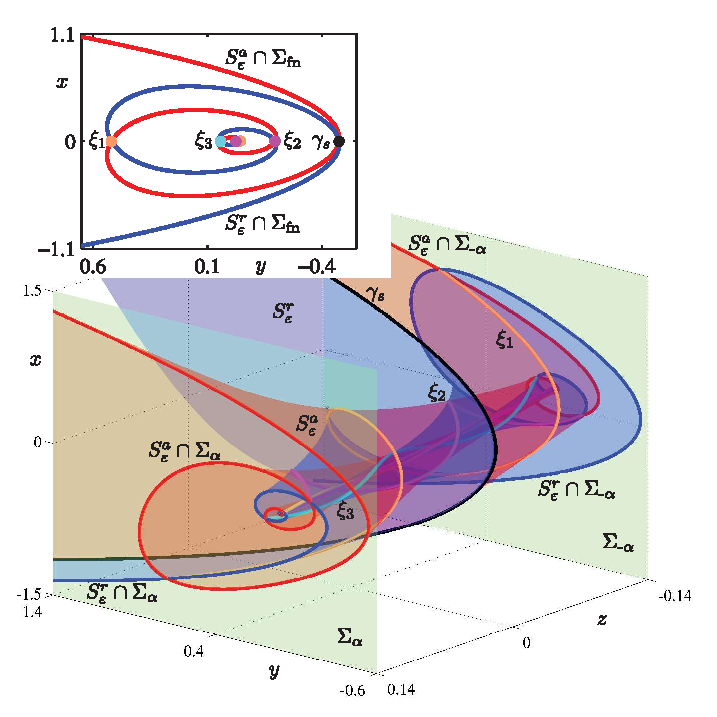
\includegraphics{Images/MMO-spirals}
	\caption{Folded Node Region for $\mu \approx0.0557$. \citep{MMO}.}
	\label{fig: MMo1pic}
\end{figure}

\begin{figure}[h!]\centering
	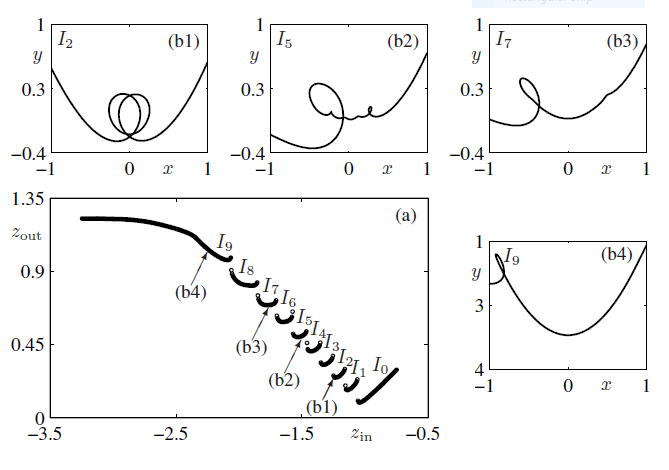
\includegraphics{Images/MMO2}
	\caption{Rotational Sectors for $\mu \approx 0.0557$ \citep{MMO}.}
	\label{fig: MMo2pic}
\end{figure}


An illustrative example is provided in \citep{MMO}, where $ \mu \approx 0.0557$ and therefore $k=8$. Then, besides the strong and weak primary canards $\gamma_s$ and $\gamma_w$, there exist eight secondary canards $\xi_i$, where $ i \in 1,...,8$.
Figure \ref{fig: MMo1pic} shows a small region of the phase space, which captures the intersection of the repelling and attracting sheet of the slow manifold. This region is bounded by two cross-sections, $\Sigma^a$ and $\Sigma^{-a}$.
Another cross-section $\Sigma^{fn}$ can be defined, which corresponds to a two dimensional cross-section of the flow at the fold. This is displayed in Figure \ref{fig: MMo1pic}. In the figure, the primary strong canard is illustrated in black, and the three strongest secondary canards are displayed as $\xi_1$ in orange, $\xi_2$ in magenta and $\xi_3$ in cyan. It is apparent that the primary strong canard makes  twists around the center, where the weak canard is located. The secondary canards $\xi_i$, $ i \in 4,...,8$ as well as $\gamma_w$ are also present. However, they are not visible since they are increasingly close to each other in the middle.\\

The number of SAOs a trajectory undergoes is dependent on where it enters the funnel region in terms of the space variable $z$. The intervals that can be defined are $I_0$ up to $I_9$, where $I_0$ is bounded by $\gamma_s$ and much larger than the other intervals. The interval $I_i$, $i \in 1, ..., 8$ is bounded by the corresponding number of secondary canards $\xi_i$ to the left and $\xi_{i-1}$ to the right, and entering the fold region through the $ith$ interval corresponds to $i$ oscillations a trajectory undergoes. This is illustrated in Figure \ref{fig: MMo2pic}

This is only a very local picture of the dynamics present in system (\ref{normalform2}). Aspects of the global analysis are presented in the following section.
